\section*{Multiple-choice}\label{sec:mc}

Dine svar skal indtastes i ITX-systemets multiple-choice modul.

\multiplechoicestart



\spoergsmaal{Arrays}
Lad \(A[0:4] = \langle 8, 2, 9, 5, 4 \rangle\) og \(B[1:5] = \langle 5, 4, 1, 2, 3 \rangle\).
Hvad er \(A[3 \cdot B[4]-3]\)?
\etsvar

\mulighederstart
\svar \(2\)
\svar \(4\)
\svar \(5\) \korrekt
\svar \(8\)
\svar \(9\)
\mulighederslut
\forklaring{
  Vi finder først \(B[4]\), som er \(2\).
  Derefter finder vi \(A[3 \cdot B[4] - 3] = A[3] \),
  som er \(5\).
}

\spoergsmaal{Toppunkter i array}
Hvilke indekser er toppunkter i følgende array: \(A[0:4] = [2,8,8,9,1]\)?
Husk at et index \(i\) er et toppunkt, hvis \(A[i]\) er større end eller lig alle naboelementer (hvert element har ét eller to naboelementer).
\fleresvar
\mulighederstart
\svar \(0\)
\svar \(1\) \korrekt
\svar \(2\)
\svar \(3\) \korrekt
\svar \(4\)
\mulighederslut
\forklaring{
  Her er \(A[1]=8\) større end \(A[0]=2\) og lig \(A[2]=8\),
  og \(A[3]=9\) større end \(A[2]=8\) og \(A[4]=1\).
  Derfor er \(1\) og \(3\) toppunkter.
}

\spoergsmaal{Kombinatorik}
Hvor mange forskellige måder kan vi vælge \(k\) elementer fra en mængde med
\(n\) elementer, når rækkefølgen ikke betyder noget og vi ikke må vælge det samme element
flere gange?
\etsvar
\mulighederstart
\svar \(n^{k}\)
\svar \(\frac{n!}{(n-k)!}\)
\svar \(\frac{n!}{(n-k)!k!}\) \korrekt
\svar \(n \cdot \sum_{i=1}^{k} i\)
\mulighederslut
\forklaring{
Det rigtige svar svarer til binomialkoefficienten \(\binom{n}{k} = \frac{n!}{(n-k)!k!}\), som præcis er antallet af delmængder af størrelse $k$ af en mængde af størrelse $n$.
}


\spoergsmaal{Hashing}
Hvilke af følgende egenskaber er gode for en hash-funktion at have?
\fleresvar
\mulighederstart
\svar Enhver nøgle (key) har samme sandsynlighed for at blive sendt til enhver indgang (entry) i hash-tabellen, uafhængigt af hvor andre nøgler sendes. \korrekt
\svar Hash-funktionen er kontinuert.
\svar Hvis man udregner hash-værdien med den samme nøgle flere gange, 
får man næsten altid forskellige resultater.
\svar Hash funktionen er hurtig at beregne. \korrekt
\mulighederslut
\forklaring{
\begin{enumerate}

    \item Vi vil gerne have en jævn fordeling af nøgler i hash-tabellen, og at nøglernes placeringer ikke afhænger af hinanden,
så vi vil gerne have egenskab (1).
\item Vi får ikke noget ud af kontinuitet i en hash-funktion,
så (2) er irrelevant. 
\item En hash-funktion skal altid give det samme resultat for den samme nøgle,
så (3) er forkert.
\item Endelig vil vi gerne have at hash-funktionen er hurtig at beregne,
så (4) er korrekt.
\end{enumerate}
}


\spoergsmaal{Begreber i grafer}
Hvilke af nedenstående begreber kan man bruge til at beskrive dele af en graf $G=(V,E)$?
\fleresvar
\mulighederstart
\svar Kanter (edges) \korrekt
\svar Cykler (cycles) \korrekt
\svar Akser (axes)
\svar Stier (paths) \korrekt
\svar Kurver (curves)
\svar Funktioner (functions)
\mulighederslut
\forklaring{
En graf består af knuder og kanter.
Man kan også tale om stier og cykler i en graf.
Begreber som akser, kurver og funktioner hører ikke til den grundlæggende grafteori.
}


\spoergsmaal{Basale pseudokode-ord}
Hvilke af følgende ord bruger vi ofte i pseudokode?
\fleresvar
\mulighederstart
\svar if \korrekt
\svar can
\svar for \korrekt
\svar return \korrekt
\svar invert
\svar align
\mulighederslut
\forklaring{
I standard pseudokode bruger vi ofte if, for og return, men ikke de andre ord.
}

\spoergsmaal{Datastrukturer fra pensum}
Hvilke af følgende er navne på datastrukturer fra kursets pensum?
\fleresvar
\mulighederstart
\svar udvidet pointer (extended pointer)
\svar kø (queue) \korrekt
\svar samling (collection)
\svar dobbelt kæde (double chain)
\svar familie (family)
\svar enkelthægtet liste (singly linked list) \korrekt
\mulighederslut
\forklaring{
Enkelthægtet liste og kø er klassiske datastrukturer i pensum. Ord som udvidet pointer, samling, dobbelt kæde og familie er ikke standard datastrukturer i kurset.
}


\spoergsmaal{Egenskaber ved binære søgetræer}
Hvilke af følgende udsagn beskriver egenskaber ved et binært søgetræ (binary search tree)?
\fleresvar
\mulighederstart
\svar Hver knude (node) har nul, et eller to børn \korrekt
\svar Hver knude har to forældre
\svar For enhver knude $v$ gælder at hvis $v.left \neq \text{NIL}$, så er $v.left.key \leq v.key$ \korrekt
\svar Højden af træet (dvs.~antal kanter (edges) på den længste sti (path) fra et blad til roden) er altid $O(\log n)$, hvor $n$ er antallet af knuder
\svar Antallet af knuder i venstre deltræ under roden er altid mindre end antallet i højre deltræ
\mulighederslut
\forklaring{
Et binært søgetræ har højst to børn per knude, og venstre barns nøgle er mindre end eller lig med knudens nøgle. Antallet af knuder i venstre og højre deltræ kan variere, så der er ikke altid færre knuder i venstre deltræ. Højden er ikke altid $O(\log n)$; det gælder kun for balancerede træer.
Hver knude har netop én forælder,  undtagen roden som ingen har.
}


\spoergsmaal{Egenskaber ved relationer}
Hvilke af følgende ord beskriver en egenskab ved en relation?
\fleresvar
\mulighederstart
\svar refleksiv \korrekt
\svar indikativ
\svar biimplikativ
\svar transitiv \korrekt
\svar projektiv
\svar distributiv
\mulighederslut
\forklaring{
Ordene refleksiv og transitiv beskriver egenskaber for relationer.
Ord som indikativ, biimplikativ, projektiv og distributiv er ikke standardegenskaber for relationer.
}


\spoergsmaal{Symmetrisk relation}
Lad $X$ være en mængde og lad $R \subseteq X \times X$ være en relation på $X$.
Hvad er definitionen på at $R$ er symmetrisk?
\etsvar
\mulighederstart
\svar Hvis $(a,b) \in R$, så er $(a,a) \in R$
\svar Hvis $(a,b) \in R$, så er $(a,c) \in R$ for alle $c \in X$
\svar Hvis $(a,b) \in R$, så er $(b,a) \in R$ og $a \neq b$
\svar Hvis $(a,b) \in R$, så er $(b,a) \in R$ \korrekt
\mulighederslut
\forklaring{
En relation $R$ er symmetrisk, hvis for alle $a,b \in X$ gælder: $(a,b) \in R \implies (b,a) \in R$.
De andre udsagn beskriver ikke symmetri.
}

\spoergsmaal{Asymptotisk analyse}
Betragt funktionen
\begin{align*}
  f(x) = x^{3}\log x + 7x^{2} + 10x.
\end{align*}
Hvilke af følgende udsagn om \(f\) er korrekte?
\fleresvar
\mulighederstart
\svar \(f = O(x^{3})\)
\svar \(f = O(x^{3}\log x)\) \korrekt
\svar \(f = O(x^{4})\) \korrekt
\svar \(f = \Omega(x^{3})\) \korrekt
\svar \(f = \Omega(x^{4})\)
\svar \(f = \Theta(x^{3}\log x)\) \korrekt
\svar \(f = \Theta(x^{3})\) 
\mulighederslut
\forklaring{
  Det dominerende led i \(f\) er \(x^{3}\log x\),
  så \(f = O(x^{3}\log x)\) og \(f = O(x^{4})\).
  Da \(f\) vokser hurtigere end \(x^{3}\) er \(f = \Omega(x^{3})\).
  Da den dominerende term er \(x^{3}\log x\) er \(f = \Theta(x^{3}\log x)\).
}

\spoergsmaal{Pseudokode}
Betragt følgende pseudokode
\begin{codebox}
\Procname{$\proc{While-Loop}(x)$}
\li $y \gets 2 \cdot x$
\li $S \gets 0$
\li \While $y > 1$ \Do
\li \(S \gets 2 \cdot S + y\)
\li \(y \gets y-2\)
    \End
\li \Return S
\end{codebox}
Hvad returneres når koden kaldes med input $x=3$?
\etsvar
\mulighederstart
\svar 3 
\svar 12
\svar 25
\svar 34 \korrekt
\svar 42
\mulighederslut
\forklaring{Vi får før whileloopet er $y=6$ og $S=0$. Herefter sker følgende i hver iteration:
\begin{itemize}
    \item Iteration 1: $S=0\cdot 2+6=6$, $y=6-2=4$
    \item Iteration 2: $S=6\cdot 2+4=16$, $y=4-2=2$
    \item Iteration 3: $S=16\cdot 2+2=34$, $y=2-2=0$
\end{itemize}
}

\spoergsmaal{RAM-model}
%TODO:Finish this one
Hvilke af følgende operationer har konstant tidskompleksitet i RAM-modellen?
Antag at \(a,b\) er heltalsvariabler og \(A\) er et array.
\fleresvar

\mulighederstart
\svar \(b = \sum_{i=1}^{n} A[i]\)
\svar \(b - a\) \korrekt
\svar \(b = A[3]\) \korrekt
\svar \(b = A[a^{3}]\) \korrekt
\svar \(b = A[b^{a}]\)
\mulighederslut
\forklaring{
  \begin{itemize}
      \item  Den første operation har tidskompleksitet \(O(n)\), da både addition og tabelopslag skal udføres \(n\) gange.
      \item  En subtraktion har konstant tidskompleksitet \(O(1)\).
      \item Et enkelt opslag i $A$ tager $O(1)$ tid.
      \item  \(a^{3}\) er et konstant antal multiplikationer, så opslaget $A[a^3]$
        har også konstant tidskompleksitet \(O(1)\).
      \item  \(b^{a}\) kan tage \(\log a\) multiplikationer i værste tilfælde.
  \end{itemize}
}




\spoergsmaal{Mængder og heltal}
Lad $A = \{5, 10, 2026\}$ og $B = \{5k \mid k \in \{1,\dots,500\}\}$.  
Hvilke af følgende udsagn er sande?
\fleresvar
\mulighederstart
\svar $\sum_{a \in A} a = 2041$ \korrekt
\svar $\text{GCD}(B) = 2500$
\svar $\sum_{b \in B-A} b=\sum_{b \in B} b-\sum_{a \in A} a$
\svar $A \subseteq B$
\svar $\sum_{b \in B} b = 5\cdot 250\cdot 501$ \korrekt
\mulighederslut
\forklaring{
$\sum_{a \in A} a=5+10+2026=2041$.
$\text{GCD}(B)=5$.
$\sum_{b \in B-A} b=\sum_{b \in B} b-5-10$, vi skal ikke trække 2026 fra som vi gør i udtrykket $\sum_{b \in B} b-\sum_{a \in A} a$.
Da $2026\notin B$ har vi ikke $A \subseteq B$.
Vi har $\sum_{b \in B} b=\sum_{k=1}^{500} 5k=5\sum_{k=1}^{500} k=5\cdot 250\cdot 501$.
}

\spoergsmaal{Modulo-beregning}
Vi minder om at for heltal $a$ og $n$ bruger vi notationen $a\text{ mod }n$ til at betegne restklassen af \(a\) modulo \(n\).
Hvad er værdien af følgende udtryk?
\begin{align*}
  (58\text{ mod }8) \cdot \left((5214\text{ mod }4)+ (8627\text{ mod }5)\right)
\end{align*}
\etsvar
\mulighederstart
\svar \(0\) 
\svar \(2\)
\svar \(6\)
\svar \(8\) \korrekt
\svar \(10\)
\mulighederslut
\forklaring{
Vi har at \(58\text{ mod }8 = 2\), \(5214\text{ mod }4 = 2\) og \(8627\text{ mod }5 = 2\).
Så regnestykket bliver \(2 \cdot (2 + 2) = 8\).
}

\spoergsmaal{Negation af udsagn}
Hvad er negationen af følgende udsagn?
\begin{align*}
  \forall x \in X \; \exists y \in Y : y \mid x^{2}.
\end{align*}
\etsvar

\mulighederstart
\svar \(\forall x \in X \; \forall y \in Y : y \nmid x^{2}\)
\svar \(\forall x \in X \; \exists y \in Y : y \nmid x^{2}\)
\svar \(\exists x \in X \; \exists y \in Y : y \nmid x^{2}\)
\svar \(\exists x \in X \; \forall y \in Y : y \nmid x^{2}\) \korrekt
\mulighederslut
\forklaring{
  For at negere udsagnet, laves alle \(\exists\)
  om til \(\forall\) og omvendt, og den indre funktion \(y \mid x^{2}\)
  negeres, som bliver til \(y \nmid x^{2}\).
}

\spoergsmaal{Max-Heap}
Du kører BUILD-MAX-HEAP på arrayet \(A = \langle 3, 1, 6, 5, 2, 4 \rangle\).
Hvilken hob (heap) får du som resultat?
\etsvar

\mulighederstart
\svar \(\langle 6, 4, 5, 1, 2, 3 \rangle\)
\svar \(\langle 6, 5, 4, 1, 2, 3 \rangle\) \korrekt
\svar \(\langle 6, 5, 4, 3, 2, 1 \rangle\)
\svar \(\langle 6, 5, 3, 1, 2, 4 \rangle\)
\svar \(\langle 6, 3, 4, 5, 2, 1 \rangle\)
\mulighederslut
\forklaring{
  Når BUILD-MAX-HEAP køres bottom-up på arrayet, flyttes den største værdi til roden,
  og hobegenskaben sikres rekursivt for alle undertræer.
  Det endelige array bliver \(\langle 6, 5, 4, 1, 2, 3 \rangle\), hvor ingen knude
  har et barn med større værdi end sig selv.
}



\spoergsmaal{Repræsentation af hægtet liste i array}
Hvilken enkelthægtet (singly linked) liste \(L\) repræsenteres af dette array \(A\)? Pointeren \(L.\text{head}\)  (dvs.~index på det første listeelement) står i \(A[0]\).
Hvert listeelement gemmes i to nabofelter \(A[i]\) og \(A[i+1]\), hvor \(A[i]\) indeholder
nøgleværdien og \(A[i+1]\) indeholder en pointer (index) til det næste listeelement.

\begin{align*}
  A[0:10] = \langle 4, 0, 3, 7, 10, 2, 0, 8, 9, 5, \text{NIL} \rangle
\end{align*}
\etsvar

\mulighederstart
\svar \(3 \rightarrow 7 \rightarrow 8 \rightarrow 5\)
\svar \(10 \rightarrow 3 \rightarrow 8 \rightarrow 5\) \korrekt
\svar \(10 \rightarrow 2 \rightarrow 7 \rightarrow 9\)
\svar \(4 \rightarrow 3 \rightarrow 10 \rightarrow 8\)
\svar Dette array definerer ikke nogen liste.
\mulighederslut
\forklaring{
  Pointeren \(L.\text{head}\) står i \(A[0]\), så vi starter ved index \(4\).
  \begin{itemize}
    \item Ved index \(4\) står nøglen \(A[4] = 10\) og pointeren \(A[5] = 2\).
    \item Ved index \(2\) står nøglen \(A[2] = 3\) og pointeren \(A[3] = 7\).
    \item Ved index \(7\) står nøglen \(A[7] = 8\) og pointeren \(A[8] = 9\).
    \item Ved index \(9\) står nøglen \(A[9] = 5\) og pointeren \(A[10] = \text{NIL}\), så listen slutter her.
  \end{itemize}
  Derfor repræsenterer arrayet listen
  \begin{align*}
    10 \rightarrow 3 \rightarrow 8 \rightarrow 5.
  \end{align*}
}





\spoergsmaal{Cuckoo hashing}
I nedenstående hashtabel er der indsat 5 nøgler med cuckoo hashing. Hver nøgle har
to mulige positioner; pilene viser den alternative placering af hver nøgle,
så f.eks. kan \(A\) flyttes mellem position \(0\) og \(1\), \(B\) mellem \(1\) og \(2\), osv.

\begin{center}
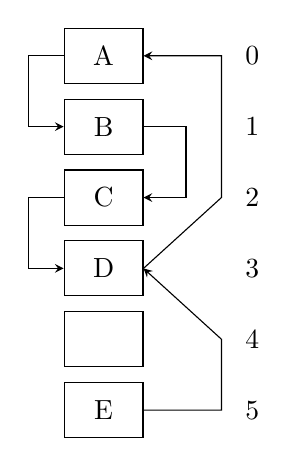
\begin{tikzpicture}[>=stealth,scale=0.9]
  \tikzstyle{slot}=[rectangle,draw,minimum width=1cm,minimum height=0.7cm,inner sep=0pt]

  % Slots (0..5)
  \node[slot] (s0) at (0,0) {A};
  \node[slot] (s1) at (0,-1) {B};
  \node[slot] (s2) at (0,-2) {C};
  \node[slot] (s3) at (0,-3) {D};
  \node[slot] (s4) at (0,-4) {};
  \node[slot] (s5) at (0,-5) {E};

  % Indices
  \node at (2.1,0) {0};
  \node at (2.1,-1) {1};
  \node at (2.1,-2) {2};
  \node at (2.1,-3) {3};
  \node at (2.1,-4) {4};
  \node at (2.1,-5) {5};

  % A: 0 <-> 1
  \draw[->] (s0.west) -- ++(-0.5,0) |- (s1.west);

  % B: 1 <-> 2
  \draw[->] (s1.east) -- ++(0.6,0) |- (s2.east);

  % C: 2 <-> 3
  \draw[->] (s2.west) -- ++(-0.5,0) |- (s3.west);

  % D: 3 <-> 0 (går opad for ikke at kollidere med E's pil)
  \draw[->] (s3.east) -- ++(1.1,1) |- (s0.east);

  % E: 5 <-> 3 (går nedenfra)
  \draw[->] (s5.east) -- ++(1.1,0) |- ++(0,1) -- (s3.east);
\end{tikzpicture}
\end{center}

Vi vil nu indsætte en ny nøgle \(K\) med mulige positioner
\begin{align*}
  h_{1}(K) = 5, \qquad h_{2}(K) = 4.
\end{align*}

Hvad er den endelige tilstand af hashtabellen efter indsættelsen af \(K\)?
\etsvar

\mulighederstart
\svar Tabellen ender som \(\langle A, B, C, D, K, E \rangle\).
\svar Tabellen ender som \(\langle D, A, B, C, K, E \rangle\). \korrekt
\svar Tabellen ender som \(\langle D, A, B, C, E, K \rangle\).
\svar Der opstår en uendelig løkke under indsættelsen, så der vil ske en rehashing.
\mulighederslut

\forklaring{
Indsættelsen forløber således:
\begin{itemize}
  \item \(K\) indsættes i position \(5\),
    så \(E\) fortrænges til sin alternative position \(3\).
  \item \(E\) indsættes i position \(3\),
    så \(D\) fortrænges til sin alternative position \(0\).
  \item \(D\) indsættes i position \(0\),
    så \(A\) fortrænges til sin alternative position \(1\).
  \item \(A\) indsættes i position \(1\),
    så \(B\) fortrænges til sin alternative position \(2\).
  \item \(B\) indsættes i position \(2\),
    så \(C\) fortrænges til sin alternative position \(3\).
  \item \(C\) indsættes i position \(3\),
    så \(E\) fortrænges til sin alternative position \(5\)
  \item \(E\) indsættes i position \(5\),
    så \(K\) fortrænges til sin alternative position \(4\)
        som er tom.
        Da \(K\) bliver indsat på en tom plads, stopper indsættelsen her.
\end{itemize}
Den endelige tabel er derfor
\begin{align*}
  \langle D, A, B, C, K, E \rangle.
\end{align*}
}


\spoergsmaal{Funktioner}
Hvilke af følgende funktioner \(f: \mathbb{R} \to \mathbb{R}\) er bijektioner?
\fleresvar

%
\mulighederstart
\svar \(x^{2}\) 

\svar \(|x|\)

\svar \(x^{3}\) \korrekt

\svar \(e^{x}\)

\svar \(2x + \sin(x)\) \korrekt
\mulighederslut
\forklaring{
  \(x^{2}\) er ikke injektiv, da \((-1)^2 = 1^2 = 1\).
  \(|x|\) er ikke injektiv da \(|-1|=|1|=1\).
  \(x^{3}\) er både injektiv og surjektiv, og dermed bijektiv.
  \(e^{x}\) er ikke surjektiv, da der ikke findes noget \( x \in \mathbb{R}\)
  så \(e^{x} < 0\).
  \(2x + \sin(x)\) er både injektiv (da den afledte er \(2 + \cos(x)\geq 1> 0\)) og surjektiv, og
  dermed bijektiv.
}


\spoergsmaal{Matrixudregning}
Lad
\begin{align*}
    A =
\begin{bmatrix}
2 & 1\\
0 & 3
\end{bmatrix},\quad
B =
\begin{bmatrix}
1 & 2\\
0 & -1
\end{bmatrix},\quad
C =
\begin{bmatrix}
0 & -2\\
0 & 2
\end{bmatrix}.
\end{align*}
Beregn udtrykket \(A B + A C\).
\etsvar

\mulighederstart
\svar \(\displaystyle
\begin{bmatrix}
2 & 1\\
0 & 3
\end{bmatrix}\) \korrekt

\svar \(\displaystyle
\begin{bmatrix}
2 & 4\\
0 & -3
\end{bmatrix}\)

\svar \(\displaystyle
\begin{bmatrix}
4 & 2\\
0 & 6
\end{bmatrix}\)

\svar \(\displaystyle
\begin{bmatrix}
1 & 0\\
0 & 1
\end{bmatrix}\)

\mulighederslut
\forklaring{
Vi kan bruge distributivitet:

\begin{align*}
    A B + A C = A(B + C).
\end{align*}

Da \(B + C = I_2\), får vi
\begin{align*}
    A(B + C) = A \cdot  I_2 = A.
\end{align*}
Altså er

\begin{align*}
A B + A C =
\begin{bmatrix}
2 & 1\\
0 & 3
\end{bmatrix}.
\end{align*}


Hvis man i stedet regner direkte:
\begin{align*}
AB =
\begin{bmatrix}
2 & 1\\
0 & 3
\end{bmatrix}
\begin{bmatrix}
1 & 2\\
0 & -1
\end{bmatrix}
=
\begin{bmatrix}
2 & 3\\
0 & -3
\end{bmatrix},
\quad
AC =
\begin{bmatrix}
2 & 1\\
0 & 3
\end{bmatrix}
\begin{bmatrix}
0 & -2\\
0 & 2
\end{bmatrix}
=
\begin{bmatrix}
0 & -2\\
0 & 6
\end{bmatrix},
\end{align*}

og dermed

\begin{align*}
    AB + AC =
\begin{bmatrix}
2 & 3\\
0 & -3
\end{bmatrix}
+
\begin{bmatrix}
0 & -2\\
0 & 6
\end{bmatrix}
=
\begin{bmatrix}
2 & 1\\
0 & 3
\end{bmatrix},
\end{align*}

}


\spoergsmaal{Pokerhænder}
Vi spiller med et almindeligt sæt på 52 spillekort (4 kulører og 13 værdier).
En hånd består af 5 kort, der trækkes tilfældigt uden tilbagelægning.
Hvor mange hænder findes der af denne type:
\begin{itemize}
\item Tre af kortene har samme værdi.
\item De resterende to kort har andre værdier, men samme kulør som hinanden.
\end{itemize}
\etsvar

\mulighederstart
\svar \(13\cdot \binom{4}{3}\cdot 4\cdot \binom{12}{2}\)\korrekt
\svar \(13\cdot \binom{4}{3}\cdot 4\cdot 12\cdot 11\) \\
\svar \(13\cdot \binom{4}{3}\cdot \binom{4}{2}\cdot \binom{12}{2}\) \\
\svar \(13\cdot \binom{4}{3}\cdot 4\cdot \binom{13}{2}\)
\mulighederslut
\forklaring{
De tre kort med samme værdi kan vælges på \(13\cdot \binom{4}{3}\) måder.
Kuløren af de resterende kort kan vælges på 4 måder, og så skal vi vælge 2 ud af de 12 resterende værdier.
Dermed får vi \(13\cdot \binom{4}{3}\cdot 4\cdot \binom{12}{2}\).
}


\spoergsmaal{Forventet Værdi}
Lad \(X_{1}, X_{2}, X_{3}, X_{4}\)
svare til resultaterne af fire uafhængige kast med en almindelig seks-sidet terning.
Hvad er den forventede værdi (expected value) af \((X_{1} + X_{2})\cdot (X_{3}+X_{4})\)?
\etsvar

\mulighederstart
\svar 24
\svar 28 
\svar 36
\svar 49 \korrekt
\svar 64 
\mulighederslut
\forklaring{Da \(X_{1} + X_{2}\) og \(X_{3} + X_{4}\) afhænger af
  forskellige terningekast, er de uafhængige, og da er den forventede værdi produktet af deres forventede værdier:
  \begin{align*}
    \mathbb{E}[(X_{1} + X_{2}) \cdot ( X_{3} + X_{4})] =
    \mathbb{E}[X_{1} + X_{2}] \cdot \mathbb{E}[ X_{3} + X_{4}] = 
    (\mathbb{E}[X_{1}] + \mathbb{E}[X_{2}]) \cdot (\mathbb{E}[ X_{3}] + \mathbb{E}[X_{4}])
  \end{align*}
  Da den forventede værdi af et enkelt kast med en seks-sidet terning er
  \begin{align*}
      \mathbb{E}[X_{i}] &=
      \frac{1+2+3+4+5+6}{6} = 3.5
  \end{align*}
  får vi resultatet 
  \begin{align*}
    \left( 3.5 + 3.5\right)^{2} = 7^{2} = 49.
  \end{align*} 
}



\spoergsmaal{Dijkstras algoritme}
Betragt den følgende vægtede, orienterede graf:

\begin{center}
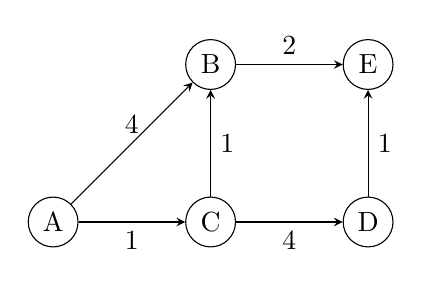
\begin{tikzpicture}[>=stealth, node distance=2.4cm]
  \tikzstyle{vertex}=[circle,draw,minimum size=18pt,inner sep=0pt]

  \node[vertex] (A) at (0,-2) {A};
  \node[vertex] (B) at (2,0) {B};
  \node[vertex] (C) at (2,-2) {C};
  \node[vertex] (D) at (4,-2) {D};
  \node[vertex] (E) at (4,0) {E};

  \draw[->] (A) -- node[above] {4} (B);
  \draw[->] (A) -- node[below] {1} (C);
  \draw[->] (C) -- node[right] {1} (B);
  \draw[->] (C) -- node[below] {4} (D);
  \draw[->] (B) -- node[above] {2} (E);
  \draw[->] (D) -- node[right] {1} (E);
\end{tikzpicture}
\end{center}

Antag Dijkstras algoritme anvendes til at finde korteste afstande fra knuden \(A\)
til alle knuder i grafen. Angiv i hvilken rækkefølge knuderne bliver taget ud af
prioritetskøen i Dijkstras algoritme.
\etsvar

\mulighederstart
\svar \(A C B E D\) \korrekt
\svar \(A B C E D\)
\svar \(A C B D E\)
\svar \(A C D B E\)
\mulighederslut
\forklaring{
  \begin{itemize}
      \item Start: \(d(A)=0\), alle andre \(\infty\).  
      \item Fra \(A\): \(d(B)=4\), \(d(C)=1\). Næste knude er \(C\) (mindst afstand).  
\item Fra \(C\): \(d(B)\) forbedres til \(1+1=2\), \(d(D)=1+4=5\).  
\item Næste knude er \(B\) (afstand \(2\)), som giver \(d(E)=1+1+2=4\).  
\item Næste knude er \(E\) (afstand \(4\)).
\item Sidste knude er \(D\) (afstand \(5\)).
\end{itemize}
Rækkefølgen er derfor \(A,C,B,E,D\).
}


\spoergsmaal{Rekursion}
Betragt den følgende rekursion:
\begin{align*}
    T(0) & = 1 \\
    T(n) & = 2T(n-1) + 1 \quad \text{for } n \geq 1.
\end{align*}
Hvilke af følgende funktioner løser rekursionen?
\etsvar

\mulighederstart
\svar \(2^{n+1}-1\) \korrekt
\svar \(2n +1\)
\svar \(3 \cdot 2^{n}-1\)
\svar \(2^{n}+n\)
\mulighederslut
\forklaring{
Vi har at \(2^{0+1}-1 = 1\), så \(2^{n+1}-1\) opfylder begyndelsesbetingelsen.
Derudover ser vi at
\begin{align*}
    2^{n+1}-1 = 2 \cdot 2^{n} - 1 = 2 \cdot \left( 2^{n} - 1\right) + 1,
\end{align*}
som viser at funktionen opfylder rekursionen.
}




\multiplechoiceslut

\label{page:last}
